
Методы решения задач компьютерного зрения включают как классические подходы, так и глубокие нейронные сети.

Классические методы основываются на внутренней структуре и симметрии изображения, 
его семантике и характеристиках объектов на нем. 
Эти методы включают в себя алгоритмы обработки изображений,
 фильтрацию, выделение признаков (например, метод гистограмм градиентов или методы локтевых точек),
  шаблонное сопоставление и классификацию на основе характеристик объектов.

\textit{Определение}\textbf{Сверточные нейронные сети} (CNN)\cite{lecun1989handwritten} представляют собой класс глубоких нейронных сетей,
использующих
специально разработанных для обработки структурно связанных данных как изображения. 
Эффективность сетей связывают с их способностью автоматически извлекать иерархические признаки из входных данных.


\begin{figure}[h]
    \centering
    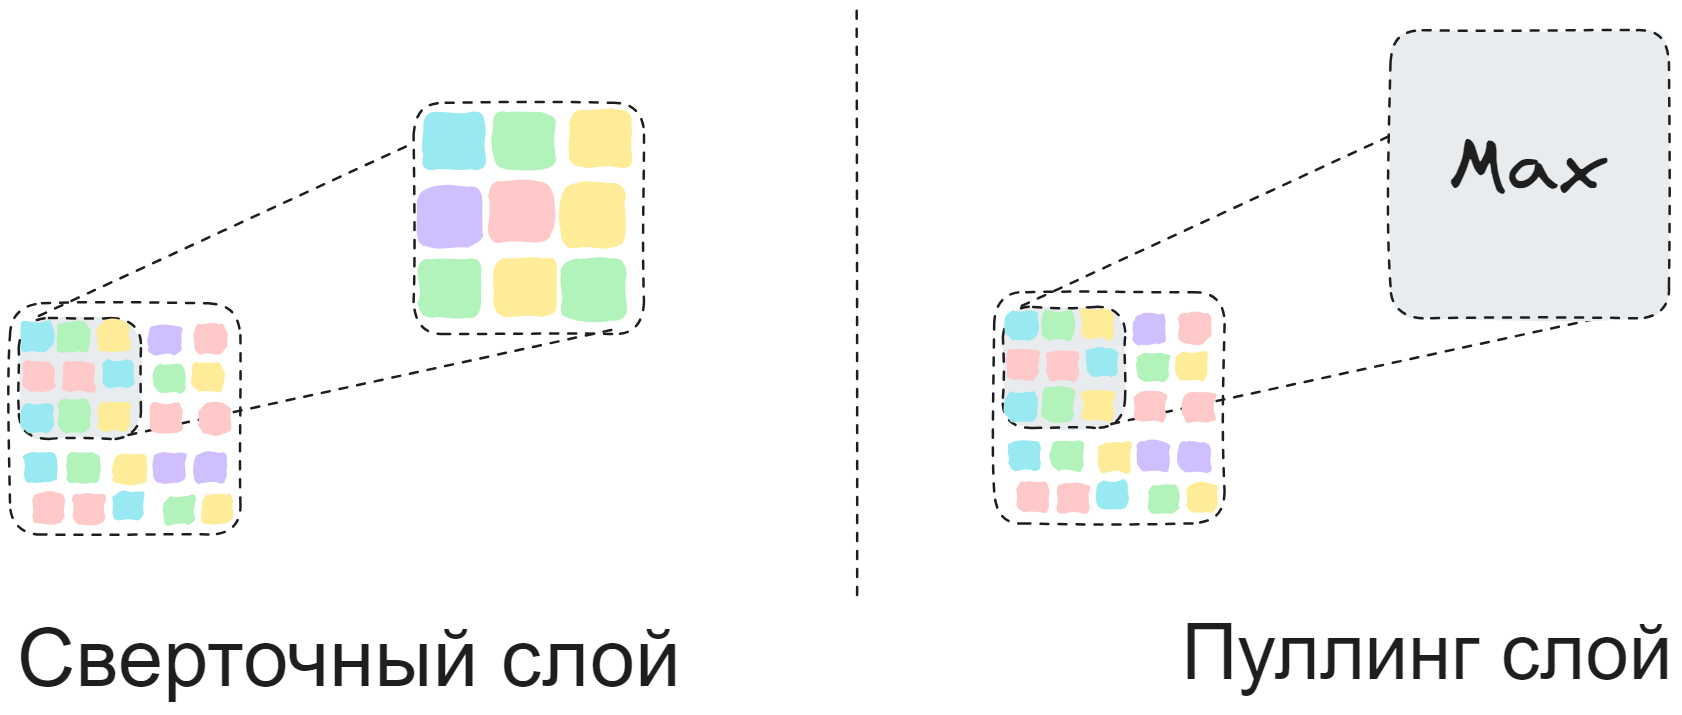
\includegraphics[width=0.5\textwidth]{assets/ml/cv/conv.excalidraw.png}
    \caption{Сверточный слой содержит параметрическое ядро, обеспечивающее выделение ключевых признаков. Пуллинг слои выполняет заранее заданную аналитическую операцию}
    \label{cnn}
\end{figure}

Глубокие методы, основанные на сверточных нейронных сетях (CNN), 
стали широко распространенными и эффективными в решении задач компьютерного зрения. 
Эти методы автоматически изучают признаки изображений на различных уровнях абстракции, 
начиная от низкоуровневых признаков, таких как грани и текстуры, до высокоуровневых семантических признаков,
 связанных с объектами и их распознаванием. 
 
Основными компонентами сверточных нейронных сетей являются \begin{itemize}
    \item сверточные слои выполняют операции свертки над входными данными с использованием фильтров или ядер, 
    чтобы извлечь локальные пространственные признаки, такие как грани, углы и текстуры. 
    Это позволяет модели обнаруживать абстрактные особенности изображений на разных уровнях детализации.
    \item пулинг слои предназначены для уменьшения пространственных размеров активаций, полученных после сверточных операций, путем объединения значений пикселей в заданных областях. 
    Это позволяет модели быть инвариантной к небольшим трансляциям объектов на изображении и уменьшает количество параметров, 
    что способствует предотвращению переобучения и повышению эффективности вычислений.
    \begin{equato}
    \item полносвязанные слои обычно располагаются в конце архитектуры нейронной сети и используются для объединения высокоуровневых признаков, 
    извлеченных предыдущими слоями, в предсказания или классификации.
\end{itemize}
 
Во время обучения сверточной нейронной сети параметры каждого слоя оптимизируются с использованием методов оптимизации, таких как обратное распространение ошибки и стохастический градиентный спуск, с целью минимизации заданной функции потерь. Этот процесс позволяет модели настраивать свои параметры для эффективного извлечения признаков и выполнения конкретной задачи, такой как классификация изображений или сегментация объектов.

\begin{figure}[h]
    \centering
    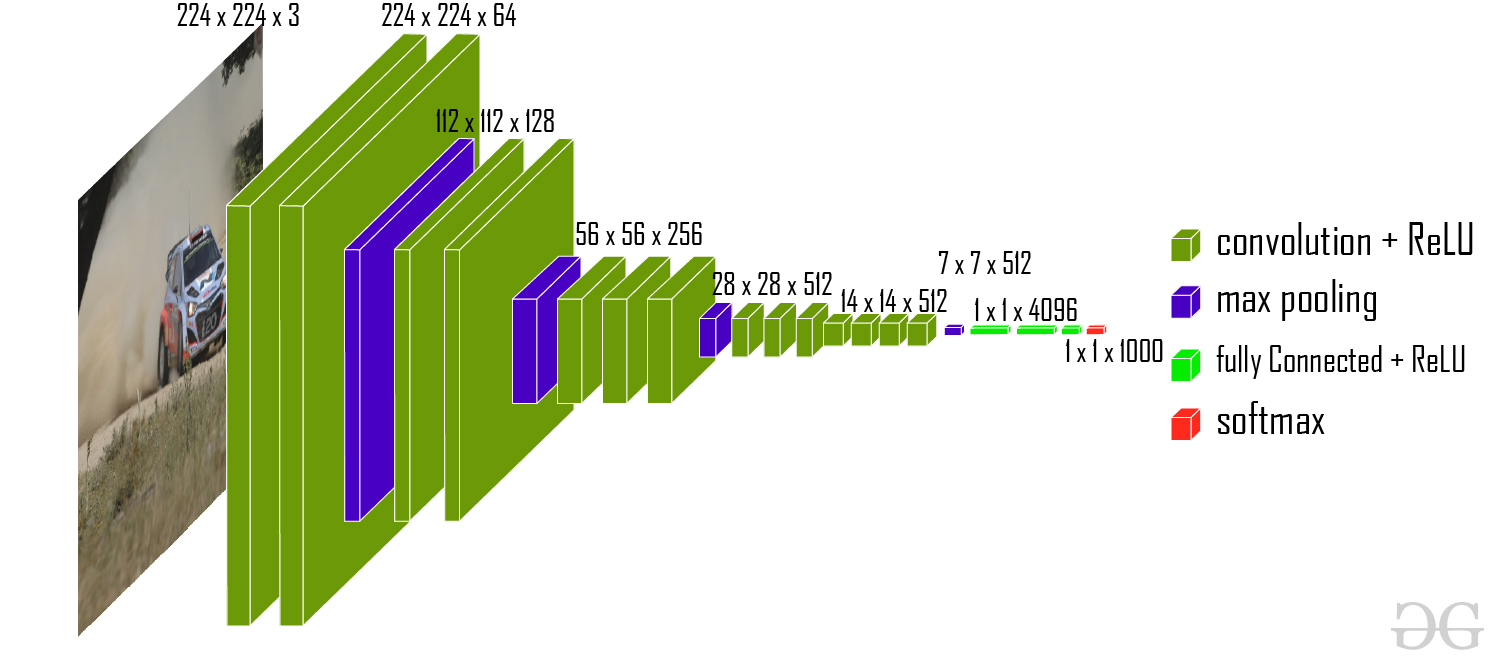
\includegraphics[width=0.5\textwidth]{assets/ml/cv/vgg16.jpg}
    \caption{Архитектура VGG16 \cite{simonyan2014very}}
    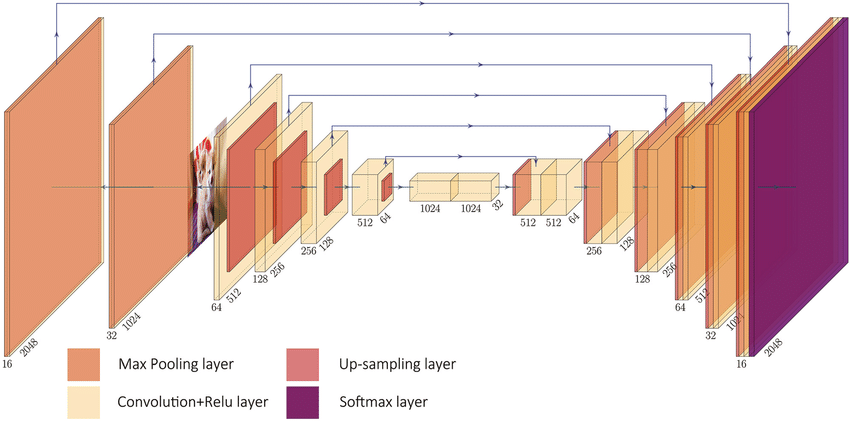
\includegraphics[width=0.5\textwidth]{assets/ml/cv/unet.png}
    \caption{Архитектура Unet \cite{ronneberger2015u}}
    \label{vgg_arch}
\end{figure}


Архитектуры U-Net  и ResNet \ref{vgg_arch} привнесли 
существенные модификации в оригинальный архитектуры сверточных сетей \begin{itemize}
    \item использование симметричной структуры, 
    включающие деконволюционные слои (upsampling) для восстановления пространственного разрешения
    \item блоки с пропуском, обеспечивающие плавное обучение глубоких сетей
    \begin{equation}
        x_{t+1} = x_t + \text{x_t}
    \end{equation}
\end{itemize}

Методы аугментации изображений в компьютерном зрении представляют собой техники,
используемые для увеличения размера и разнообразия тренировочного набора данных путем применения различных преобразований к изображениям. 
Целью аугментации является создание дополнительных вариаций изображений, что помогает улучшить обобщающую способность моделей машинного обучения и уменьшить риск переобучения.

Основные методы аугментации включают в себя
\begin{itemize}
    \item изменение размера изображения (путем масштабирования)
    \item  повороты и отражения 
    \item  изменение яркости, контраста и насыщенности цвето
    \item добавление шума или размытия.
\end{itemize}    
    
Дополнительно, могут применяться специфические трансформации, такие как сдвиги, обрезки или изменение геометрии изображения.

Применение методов аугментации позволяет модели машинного обучения обучаться на более разнообразных данных, 
что способствует повышению их устойчивости к различным условиям и изменениям в данных во время работы.
Кроме того, аугментация может помочь справиться с проблемой несбалансированных классов и улучшить обобщающую способность моделей.

Модель YOLO (You Only Look Once) представляет собой популярную архитектуру для обнаружения объектов на изображениях. Е
е основной идеей является выполнение обнаружения объектов и классификации в одной сети, что делает ее быстрой и эффективной.
\cite{kirillov2023segment}
Порядок работы модели YOLO начинается с входного изображения, которое подается на вход нейронной сети. Затем изображение проходит через сверточные слои, которые извлекают признаки из изображения на различных уровнях абстракции.

Далее, полученные признаки пропускаются через сверточные слои, которые прогнозируют боксы (ограничивающие рамки) для объектов и их вероятности принадлежности к различным классам. Эти сверточные слои производят прогнозы на основе якорей (anchors), которые представляют разные размеры и соотношения сторон боксов.

После этого выполняется пост-обработка, включающая подавление неоднородных предсказаний (non-maximum suppression), чтобы получить финальные прогнозы объектов. Этот шаг удаляет лишние дубликаты и уверенно прогнозирует объекты с наибольшей уверенностью (confidence).

В результате работы модели YOLO получается набор боксов с классами и оценками уверенности, представляющих объекты, найденные на изображении. 
Эта информация может быть использована для обнаружения объектов и их классификации в реальном времени.
